
\documentclass[journal=jacsat,manuscript=article]{achemso}


%\usepackage{amsmath}
\usepackage{amssymb}


\AtBeginDocument{\let\latin\relax}
\usepackage{chemmacros}

\usepackage{chemfig}

%\usepackage[version=3]{mhchem} % Formula subscripts using \ce{}
\usepackage[version=4]{mhchem}
\chemsetup{modules={all}}

%\usepackage{chngcntr}
%\counterwithin*{react}{chapter}

\usechemmodule{reactions}
\chemsetup[reactions]{
	before-tag = R,
	tag-open = ( ,
	tag-close = )
}

\usepackage{subcaption}
\usepackage{siunitx} % SI units package
\usepackage{paralist} % Adds inline enumeration (inparaenum) or itemization (inparaitem, inparadesc)

\newcommand*\mycommand[1]{\texttt{\emph{#1}}}
\newcommand{\nox}{\ce{NO_{\rmfamily{x}}}}
\newcommand{\Mathematica}{\textit{Mathematica}\textsuperscript{\tiny\textregistered}}
\newcommand{\hnotres}{\ce{HNO3}}
\newcommand{\no}{\ce{NO}}
\newcommand{\envinox}{\text{Envi\nox\textsuperscript{\tiny\textregistered}}}
\newcommand{\odois}{\ce{O2}}
\newcommand{\ndois}{\ce{N2}}
\newcommand{\hdoiso}{\ce{H2O}}
\newcommand{\hnodois}{\ce{HNO2}}
\newcommand{\hdoisodois}{\ce{H2O2}}
\newcommand{\naoh}{\ce{NaOH}}
\newcommand{\hdois}{\ce{H2}}
\newcommand{\nhtres}{\ce{NH3}}
\newcommand{\otres}{\ce{O3}}



\author{In\^es~L.S.B.~Vilarinho}
\affiliation[deq]{CIEPQPF, Department of Chemical Engineering, University of Coimbra, Rua S\'{\i}lvio Lima, P\'olo~II, Coimbra 3030--790, Portugal.}
\altaffiliation{Current address: CICECO--Centre for Research in Ceramics and Composite Materials, University of Aveiro, Aveiro 3810-193, Portugal.}
\email{inessvilarinho@ua.pt}
\phone{+351 927563434}

\author{Belmiro~P.M.~Duarte}
\affiliation[isec]{Department of Chemical and Biological Engineering, ISEC, Polytechnic Institute of Coimbra, Rua Pedro Nunes, Quinta da Nora,Coimbra 3030--199, Portugal.}
\alsoaffiliation[deq]{CIEPQPF, Department of Chemical Engineering, University of Coimbra, Rua S\'{\i}lvio Lima, P\'olo~II, Coimbra 3030--790, Portugal.}

\author{Susana~E.F.M.~Pereira}
\affiliation[cuf]{Bondalti Chemicals, Quinta da Ind\'ustria - Rua do Amon\'{\i}aco Portugu\^es, 10, Bedu\'{\i}do, Estarreja 3860--680, Portugal.}

\author{Nuno~M.C.~Oliveira}
\affiliation[deq]{CIEPQPF, Department of Chemical Engineering, University of Coimbra, Rua S\'{\i}lvio Lima, P\'olo~II, Coimbra 3030--790, Portugal.}


\title
  {Dynamic Rigorous Modelling of the \nox~Absorption Process: Model Validation with Industrial Data and Process Responses Analyses}



\keywords{Nitric acid, \nox~emissions reduction, dynamic modelling.}

\begin{document}

\begin{abstract}

The reduction of \nox~emissions in nitric acid plants during transient regimes still remains a technologically challenging problem. Although these emissions do not violate current environmental regulations, stricter obligations are expected in the near future raising awareness for the need of optimizing \nox~absorption systems.  Herein we present a new mathematical model for the dynamics of this process that also simulates its startup operation. 
The dynamic mathematical model was implemented in \Mathematica and several initialization strategies were required to perform the simulation. 
The model was validated with industrial data and a throughout analysis was performed to the dynamic process responses during column's startup.
We verified that:
\begin{inparaenum}[(i)]
	\item a reduction of approximately \SI{15}{\percent} of the nitric acid lateral stream concentration will lead to a maximum reduction of \SI{6.1}{\percent} of the \nox~gas pressures leaving the column, thus reducing the emissions during the startup period;
	\item a decrease of the lateral stream flow rate by \SI{30}{\percent} decreases the \nox~peak by \SI{1.30}{\percent};
	\item the increase of the secondary air flow rate did not present significantly influence;
	\item lowering the lateral feed tray two trays below the reference decreases the \nox~emission by \SI{5.9}{\percent}.
	\item the combined effect of the nitric acid concentration LFT and its position revealed a maximum decrease of \SI{10.0}{\percent}.
\end{inparaenum}
The developed model can also be used to optimize the operational procedures and can be integrated with alternative technologies, like the use of \hdoisodois, to further evaluate the \nox~reduction efficiency.
Concluding, this tool evidences potential use for dynamic optimization and control and troubleshooting of existing industrial units. 

\end{abstract}


\section{Introduction}

Nitric acid production units belong to the class of mature industrial processes. 
The basic chemistry of its
synthesis has not changed in
the last hundred years and is composed of essentially three steps
\citep{EPA2012}:
\vspace{-2mm}
\begin{enumerate}
	\setlength{\itemsep}{-10mm}
	\item Ammonia combustion that occurs in the ammonia burner: \vspace{-7mm}
	\begin{reactions} 4 NH3(g) + 5 O2(g) -> 4 NO(g) + 6 H2O(g)  "\label{rx:NH3comb}"	 \end{reactions} 
	\item Nitric oxide oxidation that occurs along the tubes:
	\vspace{-7mm}
	\begin{reactions}
		2 NO(g) + O2(g) -> 2 NO2(g)     "\label{rxn:NOoxid}"
	\end{reactions}
	\item Absorption of nitrogen dioxide in water that occurs in the absorption column:
	\vspace{-7mm}
	\begin{reactions}
		3 NO2(g) + H2O(l) -> 2 HNO3(l) + 2 NO(g)  "\label{rxn:NO2abs}"
	\end{reactions}
\end{enumerate}
	\vspace{-7mm}
Modern nitric acid plants include an abatement system, after the absorption column that can be used to significantly reduce the nitrogen oxides emissions. 
The most used technology in such systems is the selective catalytic reduction (SCR) that converts the \nox~gases with the aid of a catalyst into \ndois~and \hdoiso~in presence of ammonia as a reducing agent. 
However,
 during transient regimes these SCR systems cannot be used, since they may lead to the formation of explosive byproducts (ammonia nitrite and nitrate) -- resulting in the release the \nox~gases to the atmosphere.
The European Union specifies a limit of \SI{75}{ppmv} for \nox~emissions for new nitric acid plants, according to the Best Available Technique (BAT) Reference Document, BREF, however for about \SI{160}{\hour \per year} the plant's emission can be higher \cite{Groves2009}. 
In the United States, the limit of the \nox~emissions is approximately \SI{200}{ppmv} (0.50 pounds of \nox~per ton of 100 percent nitric acid
produced) not including the emissions during startup, shutdown and malfunction \cite{EPA2012}.
 Nonetheless, these emissions have a visual impact and may lead to formal complaints by the surrounding populations. Additionally, stricter regulations are expected in a near future, also including the transient periods, demanding alternative approaches to further reduce startup emissions. 

Although the improvement of \nox~abatement systems seems the most logical step to reduce the current gas emissions, the ``simple'' enhancement of the absorption process may also lead to significant \nox~reduction with minimal investment. 
Therefore, the development of a rigorous model capable of reproducing the steady and dynamic states of absorption units
is very appealing, since these models can be used to draw conclusions regarding their \nox~emissions.
Dynamic modelling is commonly used to improve and optimize processes. For example, \citeauthor{Schneider2001} developed a dynamic model using the two film theory to simulate a reactive absorption column, describing the reactive absorption of sour gases in a packed column. The model led to a Differential Algebraic Equations (DAE) system formed by 30,000 equations (after discretization) whose results were afterwards validated with experimental data. 
 In 2003, \citeauthor{Kenig2003} published a review on rigorous modelling of reactive absorption processes. The authors proposed a model, later validated for a set of cases, including the steady state of the \nox~absorption. In this reference, the authors state that rate-based simulations have some relevant computational complexities. Specifically, this type of models require high computational effort which may lead to numerical errors and, consequently, limit its application to industrial problems. Later, Ref.~\citenum{Kenig2009} studied the implementation of rate based models for design and control applications. The authors used the orthogonal collocation on finite elements (OCFE) technique for discretization. The simulation was implemented in gPROMS and the results were validated with experimental data from a \nox~packed column, operating at \SI{600}{\kilo\pascal} at steady state and producing a nitric acid concentration of \SI{32}{\percent}wt. The dynamic simulation was only used to demonstrate the control system response when increasing \nox~inlet concentrations.
\citeauthor{Dalaouti2005} have also developed a rate based dynamic model in gPROMS which was validated with \nox~industrial data at steady state. The proposed model predicts the dynamic response to a disturbance with different proportional-integral (PI) controllers. Several numerical tests were reported to guarantee a stable operation while controlling the \nox~emissions. Later, Ref.~\citenum{Dalaouti2006} proposed a unified model approach. This model combined a rigorous non-equilibrium rate based model with order reduction using the OCFE method. For demonstration, the authors studied a \nox~column operating at \SI{560}{\kilo\pascal} and producing \hnotres~at \SI{53}{\percent}wt.


Our framework uses the
industrial absorption column of Bondalti Chemicals as reference which is enclosed in the nitric acid
plant and promotes the absorption of nitrous oxides with water. 
Specific characteristics of this system are:
\begin{inparaenum}[(i)]
	\item operating pressures between \SI{900}{\kilo\pascal} and \SI{1400}{\kilo\pascal};
	\item production of nitric acid at \SI{68}{\percent wt.}; 
	\item presence of a lateral feed stream with weak nitric acid, approximetely \SI{40}{\percent wt.}; and
	\item existence of a cooling system placed inside the absorption unit to
	promote the release of the heat generated by the
	reactions. The column's temperature range is between \SI{293.15}{\kelvin} and \SI{323.15}{\kelvin}.
\end{inparaenum}

Considering the research work referred above as well as the complexity of the absorption process, we consider that the simulation of the \nox~absorption process, in both the steady and transient regimes, is still challenging. For a model to accurately capture the process dynamics of nitric acid formation and \nox~release, several issues need to be handle. 
Thus, we propose a rigorous mathematical model which include the following novelties:
\begin{inparaenum}[(i)]
	\item the rigorous simulation of absorption units operating near the nitric acid azeotropic conditions, \SI{68}{\percent~wt};
	\item the simulation at high pressure operation, nearly \SI{1000}{\kilo\pascal};
	\item the nitrous acid decomposition description;
	\item the consistency of the model at equilibrium conditions;
	\item the dynamic simulation of an \nox~absorption column;
	\item an effective comparison of the results with industrial data; and
	\item the simulation of a typical startup.
\end{inparaenum}
The detailed mathematical model is described in Ref. \citenum{Vilarinho2016} and in this article we present the dynamic responses of the system, analyses of the most important parameters during the nitric acid plants startup and process responses to disturbances.


\section{Rigorous Rate-based Model}

The rate-based dynamic model for the \nox~absorption in water leads to a DAE system whose form is 
\begin{subequations}
	\label{eq:daebdf}
	\begin{align}
	\label{eq:daebdf1}
	&\frac{d\bm{x}}{dt}=\bm{x}'= f(\bm{x},z,u)  \\
	\label{eq:daebdf2}
	&0=g(\bm{x},z,u)  
	\end{align}
\end{subequations}
where $\bm{x}\in \mathbb{R}^{n_d}$ stands for the vector of differential state variables, $z\in \mathbb{R}^{n_a}$ for the vector of algebraic variables, $u\in \mathbb{R}^{m}$ input variables, $\bm{x}'$ stands for the time derivative of $\bm{x}$, $f(.)\in\mathbb{R}^{n_v}$ and $g(.)\in\mathbb{R}^{n_v}$ are vectors of functions.
An important concept in the analysis of DAEs is the index of the system, commonly used as a measure of the difficulty of the numerical solution. The higher its value, the harder it is to solve the system \cite{Blajer1992,Juttner2000}.
Although several definitions can be found in the literature, the differentiation index is typically employed. Here, the index of the system is defined as the number of times the algebraic equations of the system must be differentiated in order to obtain a standard form of an ordinary differential equation (ODE) system \cite{Juttner2000}.
In our case, if the Jacobian matrix $\nicefrac{\partial g}{\partial z}$ is non-singular, the system can be converted into a set of ODEs, where the time derivative $z'=\nicefrac{dz}{dt}$ can be obtained from Equation \eqref{eq:daebdf2}.
Thus, the system of Equations \eqref{eq:daebdf} is of index-1 \cite{Brenan1996a}.
Various methods can be used for the numerical integration of these type of equations such as\cite{Blajer1992, Vilarinho2018}:  (i) Backward Differentiation Formulae (BDF) or the Gear method, (ii) Extrapolation methods, and (iii) Implicit Runge-Kutta (Orthogonal Collocation) methods, among others. Another measure of the difficulty of integration a dynamic model is the degree of stiffness.  Among the options available, the implicit BDF methods with variable order and step are widely used for this class of problems due to their good stability properties \cite{Celaya2014}. 

The numerical solution of our model is a challenging
task due to the scale of the problem, which involves about 25 000~equations, the range of operating conditions where it will be used, which
	is considerably broad, the high non-linearity and the difference in magnitude achieved by some of the
	variables.
In this study we use the model developed for the \nox~absorption column described in Ref. \citenum{Vilarinho2016}.
Note that it 
has a general structure and can be adapted to simulate
different units. 
Herein, we use the
industrial absorption column of Bondalti Chemicals for reference which is enclosed in the nitric acid
plant and promotes the absorption of nitrogen oxides with water. 

The dynamic model was implemented in \Mathematica, and the built-in NDSolve numerical routine was used to integrate the DAE system once it takes advantage of the matrix sparsity, uses symbolic manipulation, uses the high quality IDA solver, that relies on efficient BDF methods, providing numerical solutions with high accuracy and all software components are well maintained. 
The integration of DAE system requires consistent initial conditions obtained solving the steady state version of the model which requires an algebraic equation solver.

\section{Results}

The \nox~absorption column was simulated dynamically in order to evaluate its \nox~reduction capacity during nitric acid plants'startup.
All the results presented onwards are displayed in normalized scales to protect the technology licensor and the acid producer. In all cases the normalization factor used is the maximum value observed. 

\subsection{Dynamic model validation}
The dynamic model was validated comparing the simulation results with industrial data.
For this purpose, we introduced a ramp disturbance in the column's inlet pressure with a normalized slope of $3.65\times10^{-5}$ s$^{-1}$ and duration of 1440 s, keeping constant values afterwards. 

Figure \ref{fig:valdynamic} compares the model predictions with gas data collected by on-site monitoring system which  measures the \no~and \nox~pressures before the abatement reactor, hereby denoted by \envinox. 
Note that the model predicts the dynamics of the variables in the stream leaving the column, while the measurements are taken downstream. Although the residence time of the gas in the piping connecting the column to the \envinox~is small (a few seconds), the oxidation reaction of the remaining \no~still progresses, and the temperature increases approximately \SI{300}{\kelvin} due to the existing heat exchangers, changing the composition significantly due to gas equilibria.
Despite these differences, the simulation results compare fairly well with those collected from the plant.
We observe that the model response trend is similar to that measured on-site and the error is below \SI{4.70}{\percent} and \SI{3.95}{\percent} for the normalized \no~pressure, $\text{NP}_{\text{\no}}$, and the normalized \nox~pressure, $\text{NP}_{\text{\nox}}$, respectively. Therefore, our dynamic simulation reproduces well the dynamic response of the system and we believe the tool is accurate for simulating the process dynamics.
\begin{figure}[htb]
	\centering
	\begin{subfigure}{\textwidth}
		\centering
		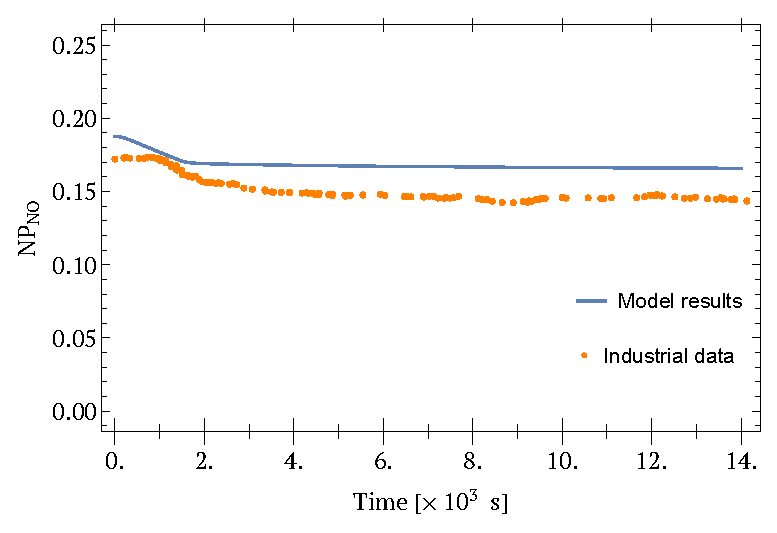
\includegraphics[width=0.6\textwidth]{figure1.eps}
		\caption{\no~in top tray} 	\label{fig:Pno31}
	\end{subfigure} 
	
	%\hspace{0.1\textwidth}%
	\begin{subfigure}{\textwidth}
		\centering
		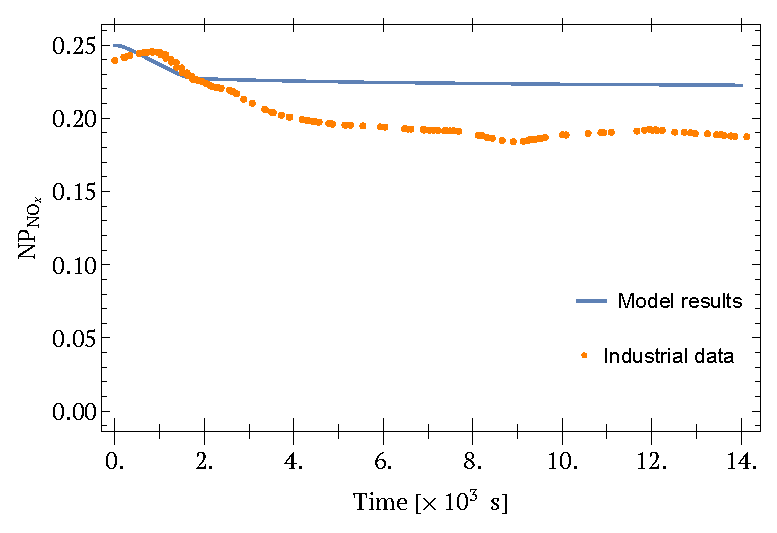
\includegraphics[width=0.6\textwidth]{figure2.eps}
		\caption{\nox~in top tray} 	\label{fig:Pno231}
	\end{subfigure}
	\caption{Responses of the leaving gas stream to an inlet pressure ramp disturbance for: (\subref{fig:Pno31}) Normalized \no~pressure  \cite{Vilarinho2018}; and (\subref{fig:Pno231}) Normalized \nox~pressure.}
	\label{fig:valdynamic}
\end{figure} 

\subsection{Column's startup simulation}
Typically, there are three different operation steps of the overall startup procedure that contribute for the \nox~emissions:
\begin{inparaenum}[(i)]	
	\item the absorption column filling;
	\item the ignition of the burner with hydrogen; and
	\item the startup of the \envinox~reactor.
\end{inparaenum}
The \nox~emissions profile during the startup is presented in  Figure~\ref{fig3} and two main peaks are observed.
The first one is caused by the filling of the absorption column with weak nitric acid, approximately \SI{40}{\percent}wt., and has a lower magnitude than the second one. This peak has already been reduced with relevant modifications in the operating conditions (as observed in the startup II results in Figure \ref{fig3}) and it will not be addressed herein.
\begin{figure}[htb]
	\centering
	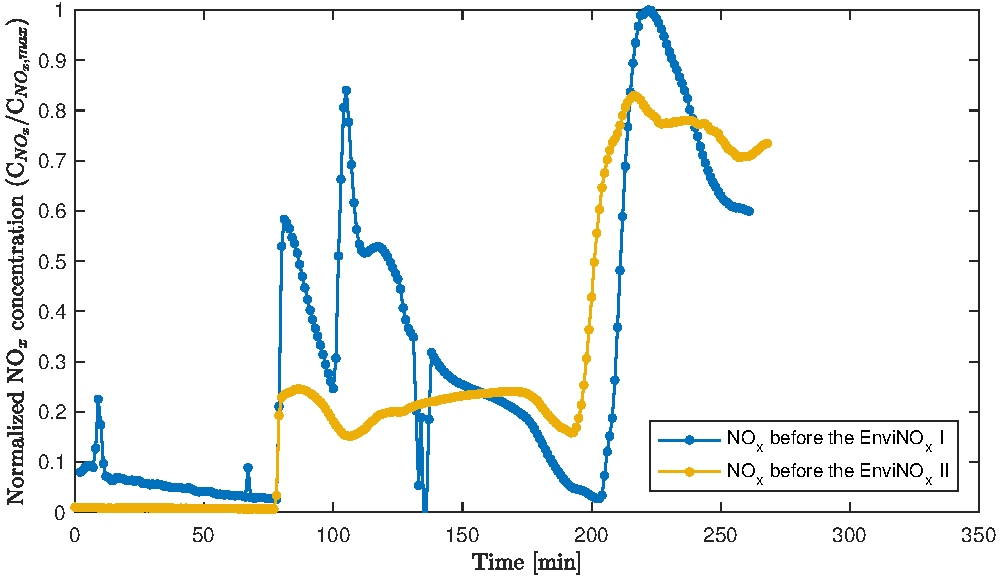
\includegraphics[width=0.8\textwidth]{figure3}
	\caption{Emissions data (before the \envinox) for two different start-ups operations.}
	\label{fig3}
\end{figure}
The second peak is caused by the ignition of the ammonia burner that forms \nox~gases and lasts up to \SI{50}{\minute}. The main cause is the inability of using the \envinox~reactor during this period due to safety problems. Consequently, the \nox~gases are not absorbed in the column and are released to the atmosphere. 


At the beginning of the column's startup, the inlet gas stream is only formed by air, and a consistent initial solution is required to solve the dynamic model for these conditions. To overcome this problem we simulated the column's steady state with the conditions used at the end of startup and imposed a negative ramp disturbance in the \nox~inlet gas stream composition.
In Bondalti Chemicals, the production rate (PR) used at the end of startup corresponds to \SI{70}{\percent}.
The comparison of plant's data and the model predictions is presented in Figure \ref{fig:wstartup}, where the points correspond to the industrial data and the black crosses to the model predictions.
Note that the data was
retrieved at different plant's relative production rates ranging from \SIrange{70}{80}{\percent}. 
The trays corresponding to smaller normalized values (left
side of the graphics and Zone~1) are those located at the bottom of
the column, and those with higher normalized values (right side of the
graphics and Zone~2) are trays at the top. The lateral feeding
stream enters the normalized tray corresponding to 0.5588. 
Our model does not include enthalpy balances because the cooling system assures that only minor gradients of temperature exist. To explicitly consider the temperature differences across the column we set a temperature profile based on on-site measurements.
The used temperature profile is that of the reference plus \SI{1}{\kelvin} (see Ref. \citenum{Vilarinho2019} for more details):
\begin{equation}
T_{n} = \begin{cases}
303.66 + 1 &  n/N_T>0.62\\
322.63+ 1 -29.75 n/N_T, \quad & 0.54 \leq n/N_T\leq 0.62 \\
307.5+ 1 & n/N_T < 0.54 
\end{cases}
\end{equation}
where $T_n$ is the temperature of tray $n$, $N_T$ the total number of trays and the reference operation corresponds to the steady state conditions attained at $\text{PR}=$\SI{95}{\percent}.
Furthermore, the
lateral feed stream enters the same tray used for $\text{PR}=95\%$,
the concentration of \hnotres~in the lateral feed stream
is \SI{1.5}{\percent} above the reference, and the operation pressure in
the column is that of the reference minus \SI{170}{\kilo\pascal} once these are the conditions obtained for $\text{PR}=70\%$.
Observing Figure \ref{fig:wstartup}, a reasonably good agreement can be noticed between the nitric acid
profile along the column and the model predictions. 
In Figure \ref{fig:wstartup} we also represented the nitric acid profile at the beginning of startup, blue crosses.
In this case we imposed a ramp that reduces the \nox~concentrations until \SI{10}{\percent} preventing numerical problems caused by null values during the initialization.   
Note that the values of the nitric acid concentrations along the column are high due to the lateral feed stream that is composed by weak nitric acid. 
\begin{figure}[htb]
	\centering
	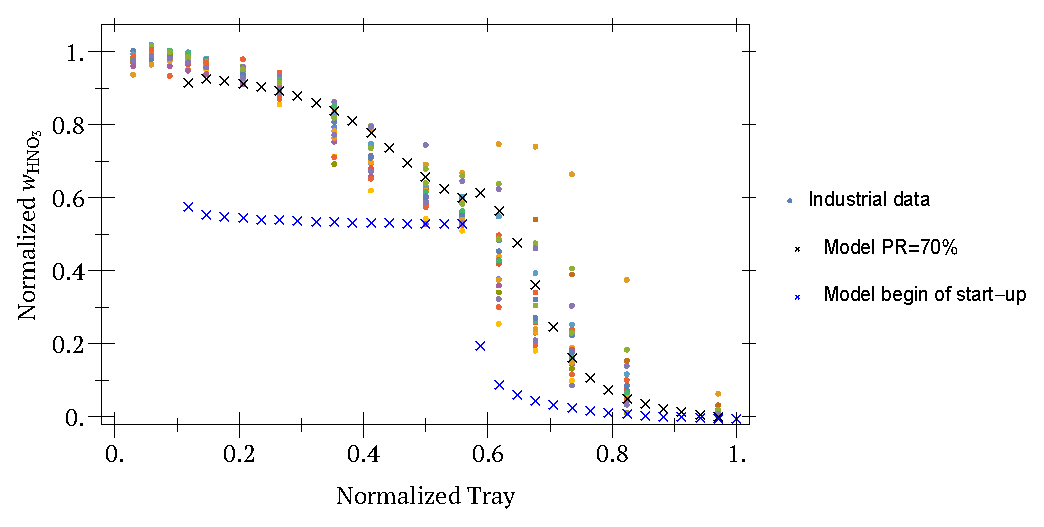
\includegraphics[width=\textwidth]{figure4.eps}
	\caption{Comparison between plant's data and model predictions for $PR=$\SI{70}{\percent}, at the beginning and end of startup.}
	\label{fig:wstartup}
\end{figure}

The Bondalti's nitric acid startup was analysed and most important operational procedures are presented concomitantly in Figure \ref{fig:sup1all} by splitting the time interval. Different ramps corresponding to feed operations are noted. In Figure \ref{fig:sup1all} the first plot corresponds to the inlet column's pressure, $NP_T$, the second one to the column's inlet water flowrate, $NL_{\text{\hdoiso}}$, the third to the secondary air flowrate, $NG_{\text{sec.air}}$ and the last one to the column's outlet \nox~pressures, $NP_{\text{\nox}}$.
Our goal of splitting the time interval is to avoid discontinuities in the mathematical model.


The number of subintervals depends on the number of explicit discontinuities of the system and, in this case, 8 subintervals are specified. In more detail, the sequence of the operations is:


\begin{enumerate}[(i)]
	\item $[t_0,t_1]$ - constant regime;
	\item $[t_1,t_2]$ - increase the water flow rate;
	\item $[t_2,t_3]$ - increase the inlet \nox~gas composition, decrease of the total absorption pressure and keep increasing the water flow rate;
	\item $[t_3,t_4]$ - keep water flow rate constant;
	\item $[t_4,t_5]$ - decrease the inlet water flow rate;
	\item $[t_3,t_6]$ - increase the total absorption pressure;
	\item $[t_2,t_7]$ - increase the secundary air flow rate; and
	\item $[t_7,t_8]$ - stabilize all variables until the steady state is reached.
\end{enumerate}

The observation of \nox~emissions at the beginning of the start up procedure reveals an increase that lasts approximately \SI{860}{\second}. After this increase there are three peaks in the \nox~pressure. Notice that the shape of the peaks is different for every analysed startup, see Ref. \citenum{Vilarinho2019}. 
We recall that the decrease of the \nox~pressure in the industrial data around 06:30 is caused by the \envinox~reactor that was started and represents the end of the nitric acid startup. After this, the plant's production rate is increased to the desired value. From this point forward, there are no major concerns regarding the gas emissions since the \nox~are abated in the \envinox~reactor.
As a result, the \nox~emissions that the company pretends to reduce are those occurring until \SI{3000}{\second}.


\begin{figure}[htb]
	\centering
	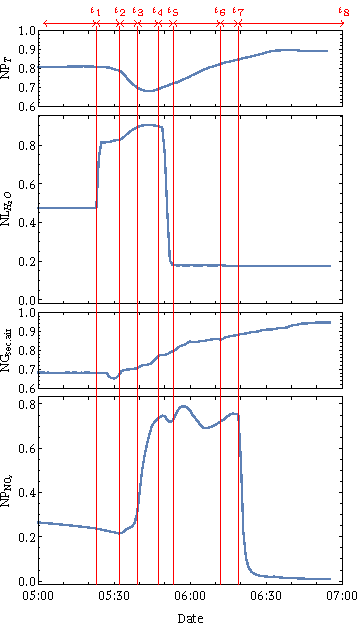
\includegraphics[width=0.7\textwidth]{figure1sp.pdf}
	\caption{Sequence of the most relevant changes during one startup operation.} 	
	\label{fig:sup1all}
\end{figure}

Together with Bondalti Chemicals, we set a reference schedule to simulate the startup of the absorption column, that are mathematical functions describing the inputs profiles captured from Figure \ref{fig:sup1all}.
The reference was established in order to generate a proper sequence of operations that allows comparing the behaviour of the unit with the model predictions. Practically, we observed a relevant variability in the analysed startup procedures, indicating a certain degree of change in the basic disturbances induced on the unit. A deeper analysis led us to consider that the startup is formed by a sequence of eight stages identified in Figure  \ref{fig:sup1all}. After this, we characterized each of the ramps forming the overall procedure, and noticed that four input variables change either simultaneously or individually:
\begin{itemize}
	\item \nox~inlet molar flow rate the sequence is: 
	\begin{enumerate}[(i)]
		\item increase with a ramp slope of 0.058 $\text{s}^{-1}$ (normalized value) from $t_1$ to $t_2$; followed by
		\item a constant value in the interval $[t_2,t_8]$.
	\end{enumerate}
	\item Column's inlet total pressure, we conceptualize the following sequence:
	\begin{enumerate}[(i)]
		\item decrease with a normalized ramp slope of $1.05 \times 10^{-4}$ $\text{s}^{-1}$ from $t_2$ to $t_3$;
		\item increase with a normalized ramp slope of $6.73 \times 10^{-5}$ $\text{s}^{-1}$ from $t_3$ to $t_6$; followed by 
		\item a period where the value is kept constant, in the interval $[t_6,t_8]$.
	\end{enumerate}
	\item Column's inlet water flow rate, the sequence includes the: 
	\begin{enumerate}[(i)]
		\item increase with a normalized ramp slope of 0.023 $\text{s}^{-1}$ from $t_0$ to $t_1$;
		\item a constant value in the interval $[t_1,t_4]$;
		\item decrease with a normalized ramp slope of 0.012 $\text{s}^{-1}$ from $t_4$ to $t_5$; and 
		\item a constant value in the interval $[t_5,t_8]$.
	\end{enumerate}
	\item Secundary air flow rate, the sequence is as follows:
	\begin{enumerate}[(i)]
		\item increase with a normalized ramp slope of $6.3 \times 10^{-6}$ $\text{s}^{-1}$ from $t_2$ to $t_7$; and 
		\item a constant value in the interval $[t_7,t_8]$.
	\end{enumerate}
\end{itemize}


Figure \ref{fig:modelall} shows the graphical representation of each modelled ramp. 


\begin{figure}[htb]
	\centering
	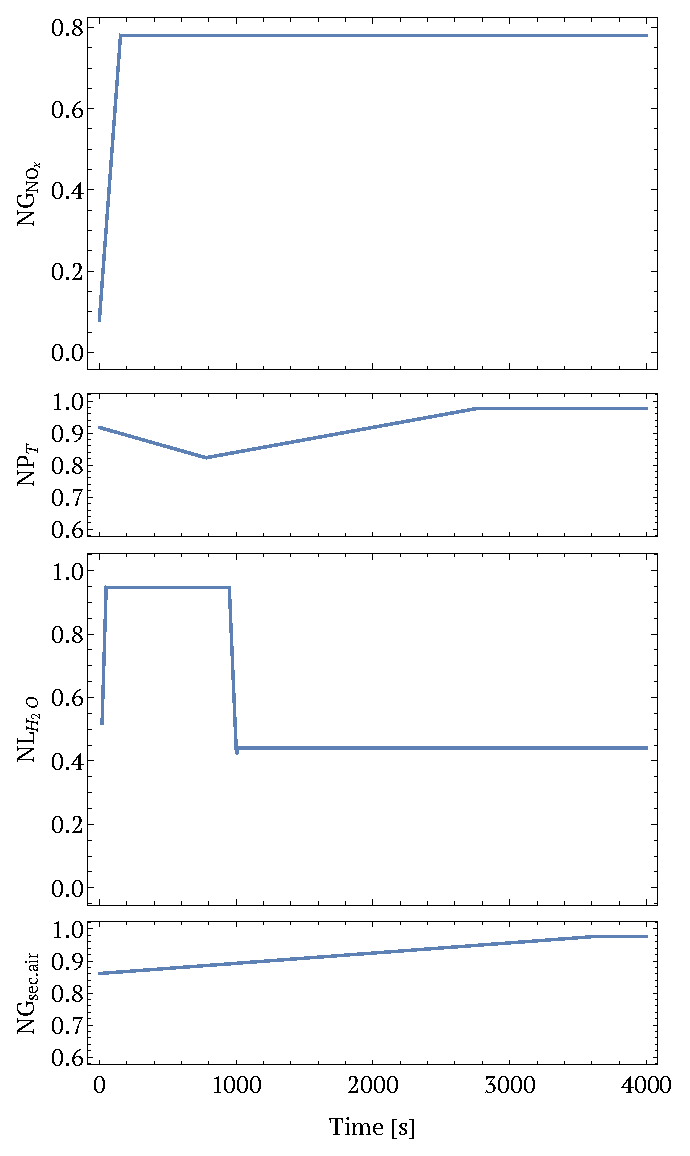
\includegraphics[width=0.7\textwidth]{figure2sp.eps}
	\caption[Sequence of ramps of the start-up procedure.]{Sequence of ramps of the start-up procedure: the first plot corresponds to the column's inlet \nox~gas flowrate, $NG_{\text{\nox}}$, the second to the inlet column's pressure, $NP_T$, the third to the column's inlet water flowrate, $NL_{\text{\hdoiso}}$, and the last one to the secondary air flowrate, $NG_{\text{sec.air}}$.} 
	\label{fig:modelall}
\end{figure}


The \nox~gas pressure leaving the column during the reference startup is presented in Figure \ref{fig:modelCUF1} together with the industrial data from one startup, where the red line represents the beginning of the abatement reactor and consequently, the \nox~pressures start to decrease.
\begin{figure}[htb]
	\centering
	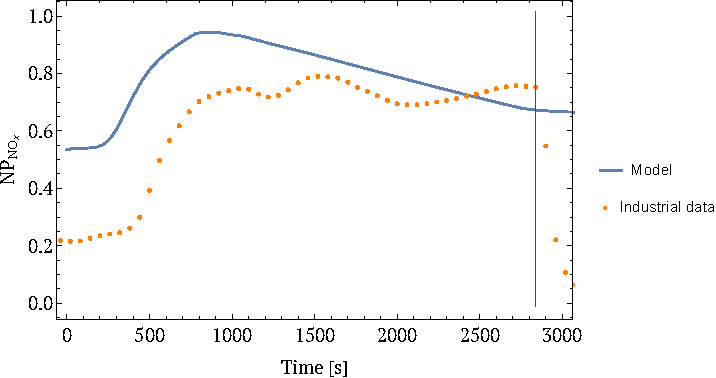
\includegraphics[width=0.8\textwidth]{figure5}
	\caption{\nox~gas pressure leaving the column during the start-up for the reference case and Start-up I.} 	
	\label{fig:modelCUF1}
\end{figure}
Figure \ref{fig:modelCUF1} shows some differences between the simulation for the reference case and the industrial data, although a similar overall trend is observed. Note that at the beginning of the start-up (0 seconds) the \nox~pressures leaving the column are not null, because we already have the influence of the lateral feed stream which cause the release of gas due to desorption. Furthermore, the observed differences between the industrial data and the model may be due to:
\begin{inparaenum}[(i)]
	\item the denitrification of the absorption column after starting the lateral feed stream. After the absorption column is filled, air passes through the column until the ignition of the burner occurs, and this will cause the denitrification of the liquid phase. This means that the industrial nitric acid profile at the beginning of this startup (orange points in Figure \ref{fig:wstartup}) is lower than the one used for simulation (blue line in Figure \ref{fig:wstartup});
	\item the different location of the \nox~pressures sampling points used for comparison (the model simulates the \nox~pressure leaving the absorption column, while on site the data was gathered after the \envinox~reactor);
	\item the assumption that the start-up occurs in the conditions that corresponds to plant's relative production rate of \SI{70}{\percent}; and
	\item the inlet gas concentrations at the beginning of the startup that is assumed to be \SI{10}{\percent} of that at the steady state conditions for PR=\SI{70}{\percent}. 
\end{inparaenum}
Nevertheless the \nox~pressure increases at the beginning of the startup and this ramp lasts for approximately \SI{780}{\second}, very close to that observed from industrial data. 
After the peak in the model predictions, the \nox~pressure decreases until a new steady state is reached. Note that this decrease coincides with the pressure increase, which has a major impact on the system.
The other peaks in the industrial data are not observed in the model prediction because the shape of the peak is different in every startup and only the main disturbances were simulated. 
However, process responses to disturbances can be analysed in order to study and optimize the process procedures in order to reduce the \nox~emissions.



\subsubsection{Process responses analyses}
The basic goal of using the dynamic model is to forecast the process behaviour when disturbances occur and gather knowledge that can help to improve the process control and the reduction of \nox~peaks during startup. For this purpose we considered the following variables:
\begin{inparaenum}[(i)]
	\item nitric acid concentration of the lateral feed stream;
	\item flowrate of the lateral feed stream;
	\item secondary air flowrate; and
	\item lateral feed tray position.
\end{inparaenum}

The nitric acid concentration of the lateral stream has a strong impact on the profiles within the column, and the lower its concentration the lower the \nox~gas pressure leaving the column \cite{Vilarinho2019}. Consequently, we analyse the transient response of the system to a disturbance in this variable. Figure \ref{fig:startw} compares the \nox~gas pressure leaving the column during the startup for the reference case, where a lateral feed stream with nitric acid mass fraction of 0.41 (reference) is used, and for a scenario where the lateral nitric acid mass fraction is 0.35.

\begin{figure}[htb]
	\centering
	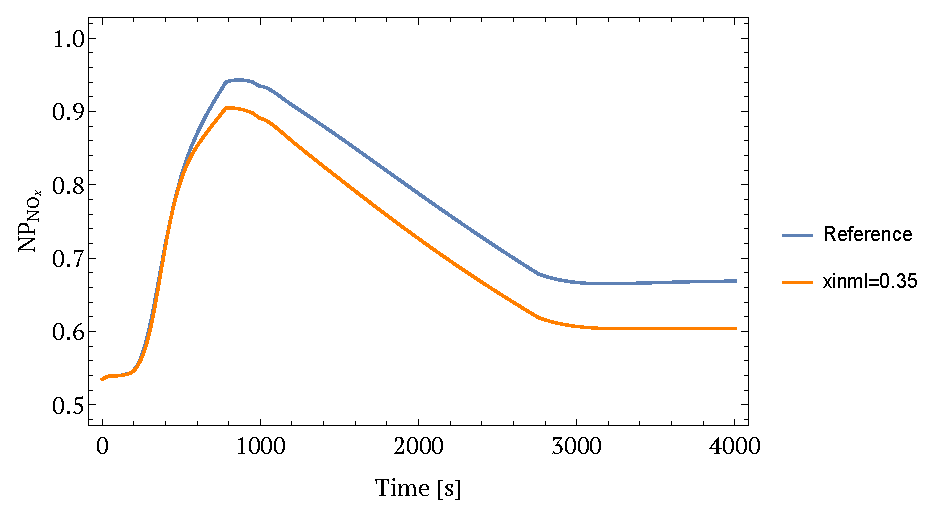
\includegraphics[width=0.8\textwidth]{figure6.eps}
	\caption{Comparison of the \nox~gas pressure leaving the column between the reference case and when the lateral feed stream nitric acid mass fraction is 0.35.} 	
	\label{fig:startw}
\end{figure}

\begin{figure}[htb]
	\centering
	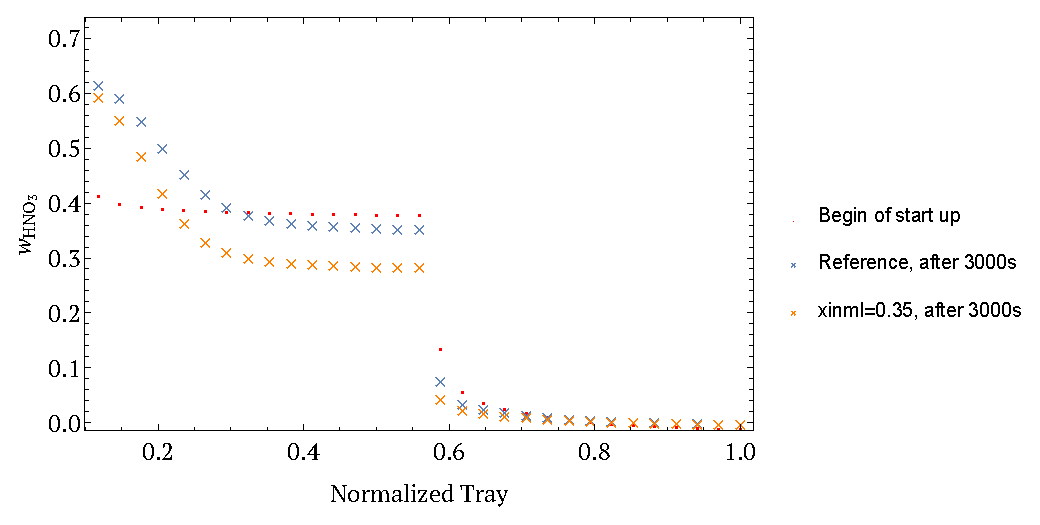
\includegraphics[width=0.8\textwidth]{figure7.eps}
	\caption{Nitric acid mass fraction profile in the absorption column at the beginning and end of the startup when lateral stream nitric acid mass fraction is reduced.} 	
	\label{fig:startwperfil}
\end{figure}
We observe that the reduction of the lateral stream nitric acid concentration will reduce the \nox~gas concentrations leaving the column. The peak is reduced by approximately \SI{3.9}{\percent}, and this decrease is extended to the whole time horizon of the simulation being approximately \SI{6.1}{\percent}, at the end.
The decrease of the \nox~gas pressures leaving the column is expected since the decrease of the nitric acid concentration in the lateral feed stream will lead to an increase of the \nox~absorption driving force in Zone 1. 
Due to safety limitations the nitric acid mass fraction cannot be lower than 0.3 below the lateral feed tray consequently, the nitric acid profile along the column at the beginning of the startup operation and after \SI{3000}{\second} is presented, see
Figure \ref{fig:startwperfil}. Here, we observed that at the end of the startup the nitric acid mass fraction in the LFT (corresponding to a normalized tray of 0.56) is lower than 0.3 being 0.286. This value can be tolerated but lower nitric acid mass fractions cannot be used. The nitric acid concentration in the first tray is not relevant during the startup procedure but we can see that it has increased, as expected, from 0.425 to 0.600. 

The effects of the lateral feed stream flow rate and secondary air flow rate during the column's startup are herein presented. Figure \ref{fig:startLinl} represents the simulation results for the reference scenario and for a scenario where the flow rate is reduced by \SI{30}{\percent}.
\begin{figure}[htb]
	\centering
	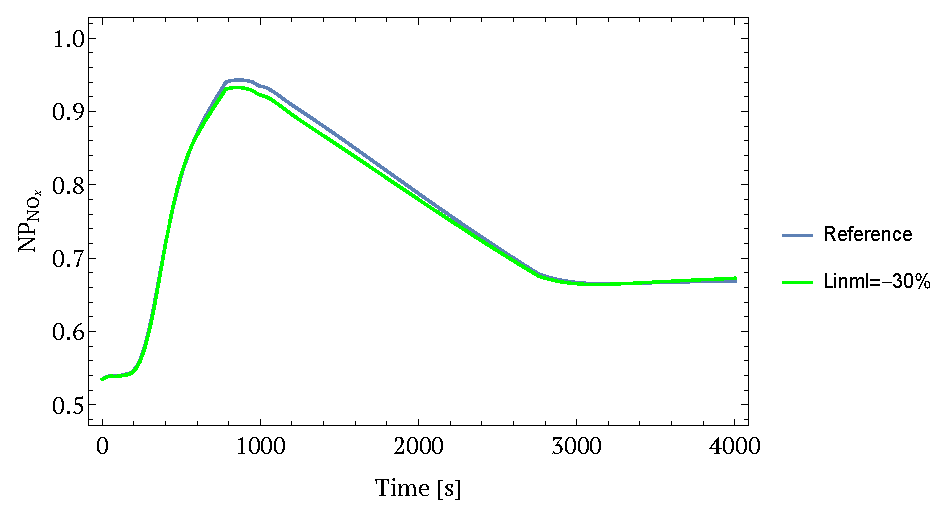
\includegraphics[width=0.8\textwidth]{figure3sp.eps}
	\caption{Comparison of the \nox~gas pressure leaving the column between the reference case and in case the lateral feed stream flow rate is reduced by  \SI{30}{\percent}.} 	
	\label{fig:startLinl}
\end{figure}
The analysis of Figure \ref{fig:startLinl} reveals that no considerable impact occurs when reducing the lateral feed stream flow rate by \SI{30}{\percent}; specifically, a decrease of \SI{1.3}{\percent} is observed at the peak. Figure \ref{fig:startLinlperfil} presents the nitric acid mass fraction profile at the beginning and end of startup. Observing the figure, we can conclude that decreasing the lateral feed stream flow rate will lead to an increase in the absorption rate in Zone 1, compared to the reference case, and consequently, the \hnotres~concentration is lower in the lateral feed tray. However this reduction is not significant and in Zone 2 the nitric acid profile is similar to that of the reference. Thus, low impact is observed in the \nox~gas stream leaving the column.


\begin{figure}[htb]
	\centering
	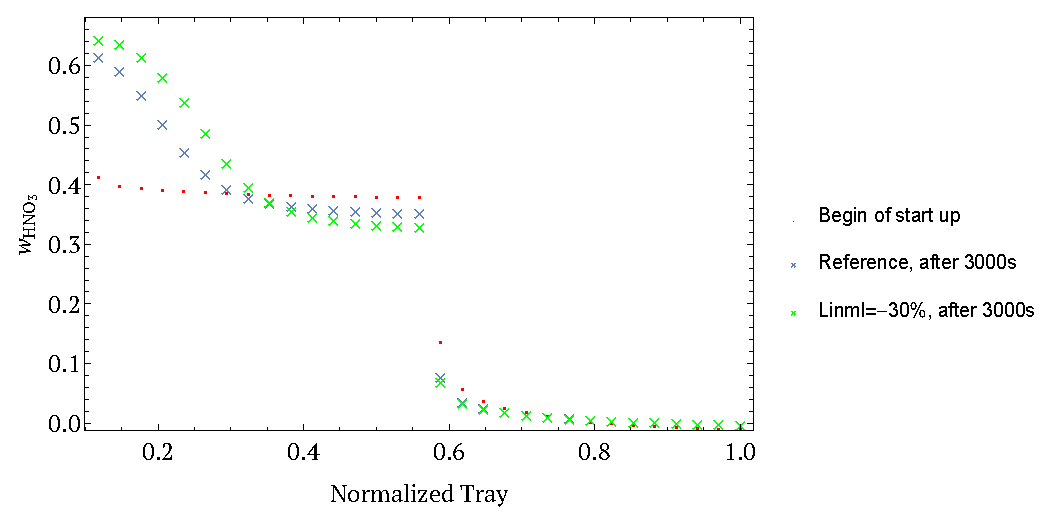
\includegraphics[width=0.8\textwidth]{figure4sp.eps}
	\caption{Nitric acid mass fraction profile in the beginning and end of startup in case the lateral stream flow rate is reduced by \SI{30}{\percent}.} 	
	\label{fig:startLinlperfil}
\end{figure}


The impact of the secondary air flow rate was also analysed, by simulating an increase of \SI{33.3}{\percent} with a normalized ramp slope of $1.6 \times 10^{-5}$ s$^{-1}$, from $t_2$ until $t_7$, as opposed to the reference scenario where an increase of \SI{13.4}{\percent} with a normalized ramp slope of $6.3 \times 10^{-6}$ s$^{-1}$ was used.
After the ramp, the secondary air flow rate was kept constant for the remaining period.
The comparison of the \nox~gas leaving the column between the reference case and this new scenario is shown in Figure \ref{fig:startair}.
\begin{figure}[htb]
	\centering
	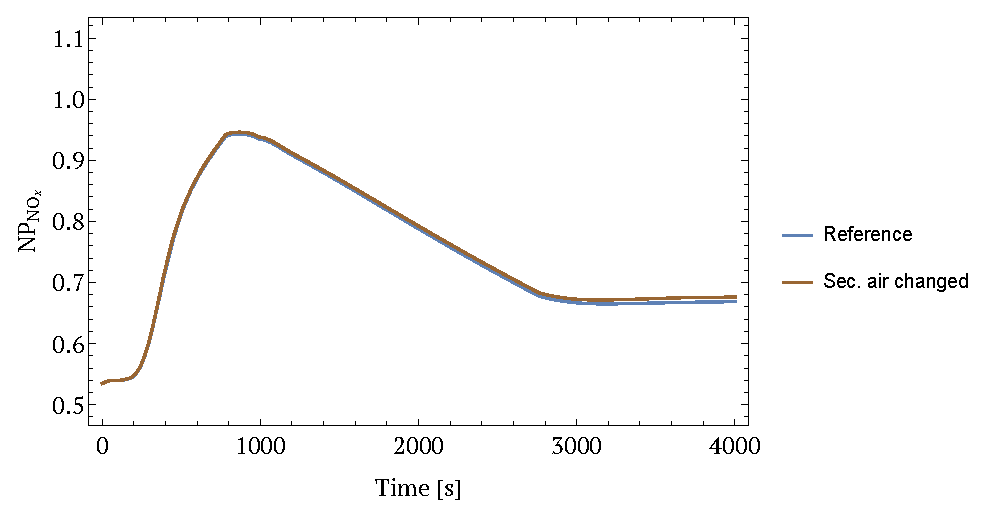
\includegraphics[width=0.8\textwidth]{figure5sp.eps}
	\caption{Comparison of the \nox~gas pressure leaving the column between the reference case and in case the secondary air has a different ramp profile.} 	
	\label{fig:startair}
\end{figure}
The dynamics do not show significant differences in the \nox~gas concentration leaving the column during the startup. 
The secondary air flow rate has an impact in the \no~oxidation rate as it increases the oxygen content in the inlet gas stream. This increase induces a higher oxidation rate which promotes the increase of the \nox~absorption rate, verified in Figure \ref{fig:startairperfil} where the beginning and end of startup profiles are analysed.

Figure \ref{fig:startairperfil} shows the influence of increasing the secondary air flow rate along the column and, in this case, no difference is observed when compared to the reference. Consequently, the increase of the secondary air does not have a significant impact on the \nox~pressures leaving the absorption column. Notice that, in this case, the mass fraction in Zone 1 is above 0.3 not causing any safety problems.

\begin{figure}[htb]
	\centering
	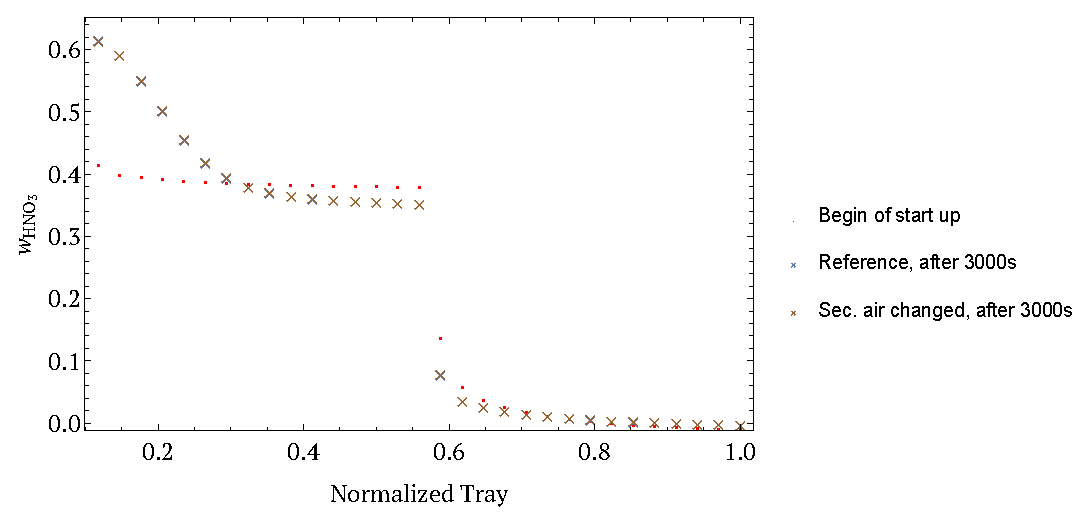
\includegraphics[width=0.8\textwidth]{figure6sp.eps}
	\caption{Nitric acid mass fraction profile in the absorption column at the beginning and end of startup in case the secondary air has a different ramp profile.} 	
	\label{fig:startairperfil}
\end{figure}

Further, the lateral feed tray position was also analysed and the results are presented in Figure \ref{fig:startp}.
\begin{figure}[htb]
	\centering
	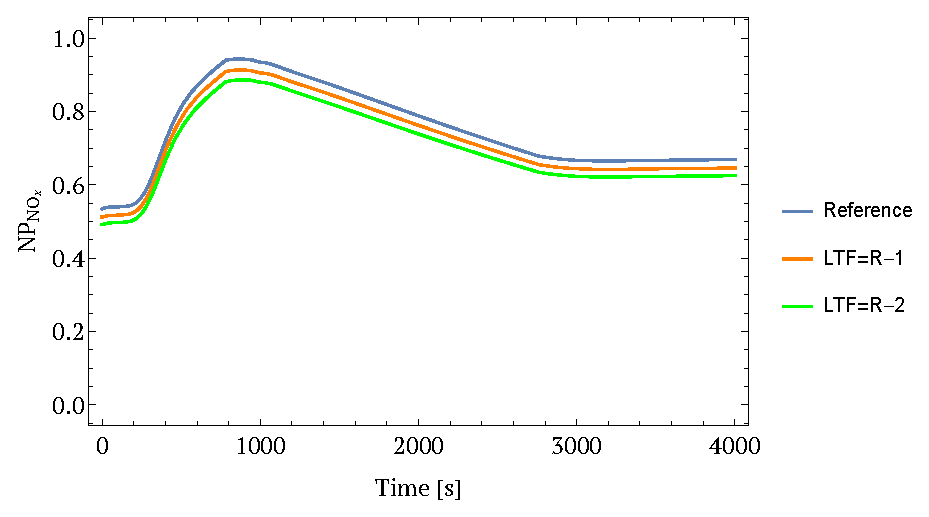
\includegraphics[width=0.8\textwidth]{figure8.eps}
	\caption{Comparison of the \nox~gas pressure leaving the column between the reference case and when the lateral feed tray is moved 1 and 2 trays below.} 	
	\label{fig:startp}
\end{figure}
Here, a decrease of \SI{3.4}{\percent} is observed at the peak and \SI{2.9}{\percent} at the end of the startup for one tray and \SI{5.9}{\percent} and \SI{5.2}{\percent}, respectively when moved the LFT two trays below.
Lowering the lateral feed position will increase the reaction volume in Zone 2 (rectifying zone) where the \nox~gases that were not absorbed in Zone 1 can be further absorbed, which was verified my the mathematical model.  

Finally, the combined effect of the nitric acid concentration at 0.35 in the LFT and its position, two trays below the reference, was studied and the total \nox~reduction is presented in the graphical figure. In this case, a decrease of \SI{8.7}{\percent} is observed at the peak and \SI{10.0}{\percent} at the end of the startup. Moreover, the simulation reveals that the effect of the disturbances on \nox~pressures is additive and both modification can be implemented simultaneously.




In summary, we present a new rigorous rate based model for the \nox~absorption process that analyse the dynamics of an absorption column and simulates a startup operation. From the model results we observed that the nitric acid plant in Bondalti Chemicals can reduce the \nox~emissions implementing some of the disturbances analysed. Furthermore, the mathematical tool presented in this work might be used to study different approaches like the use of \hdoisodois~in the absorption column and can also be applied to other units.  Concluding, the \nox~emissions in nitric acid plants during transient regimes can be reduced by optimizing plant's startup procedures. 








%%%%%%%%%%%%%%%%%%%%%%%%%%%%%%%%%%%%%%%%%%%%%%%%%%%%%%%%%%%%%%%%%%%%%
%% The "Acknowledgement" section can be given in all manuscript
%% classes.  This should be given within the "acknowledgement"
%% environment, which will make the correct section or running title.
%%%%%%%%%%%%%%%%%%%%%%%%%%%%%%%%%%%%%%%%%%%%%%%%%%%%%%%%%%%%%%%%%%%%%
\begin{acknowledgement}

The authors thank the financial support by Funda\c c\~ao para a Ci\^encia e Tecnologia (FCT) for the Ph.D. Grant SFRH/BDE/51755/2011 and by Bondalti Chemicals.


\end{acknowledgement}


%\begin{suppinfo}	
%	Description of the operational procedures during Bondalti's nitric acid startup and additional information of the dynamic process response specifically the model results for the disturbance in the flowrate of the lateral feed stream and in the secondary air flowrate.
%\end{suppinfo}

\bibliography{ACS-dynamic}




\makeatletter
\setlength\acs@tocentry@height{8.25cm}
\setlength\acs@tocentry@width{4.45cm}
\makeatother

\begin{tocentry}

\begin{center}
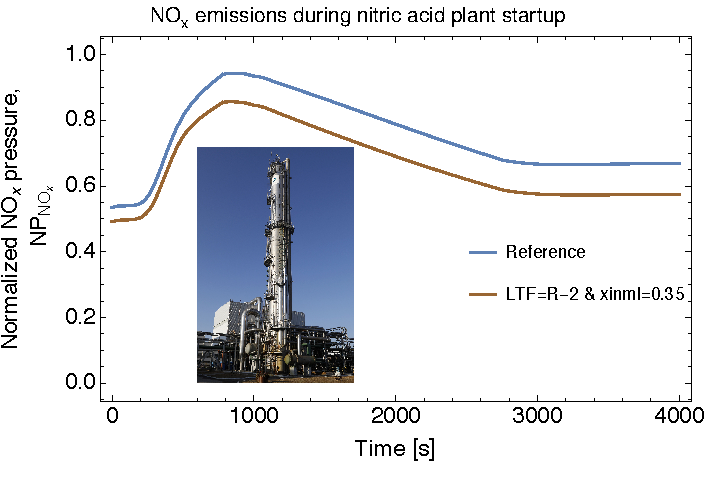
\includegraphics[width=0.865\textwidth]{graphicalfigure}
\end{center}


\end{tocentry}

%\section{Synopsis}
%The \nox~emissions in nitric acid plants during transient regimes can be reduced by optimizing plant's startup procedures. 


\end{document}
